\section{FRFs of the structure}
\label{sec:FRFs}

Once the model has been defined and the natural frequencies and mode shapes have been calculated, the next step is to compute the Frequency Response Functions (FRFs) of the structure.
The FRFs are a fundamental tool in the analysis of dynamic systems, as they provide a quantitative measure of the system's response to an external excitation as a function of frequency.

\subsection{FRFs computation}
\label{subsec:FRFs_computation}

To compute the FRFs, we can either use the direct method or the modal superposition method.

\paragraph{Direct method}

The direct method consists of solving the classical equation of motion considering all the degrees of freedom of the system (or equivalently, all the possible mode shapes of the system).

The equation of motion for a linear system can be written as:

\begin{equation}
    \mathbf{M} \ddot{\mathbf{u}} + \mathbf{C} \dot{\mathbf{u}} + \mathbf{K} \mathbf{u} = \mathbf{F}
\end{equation}

Where $\mathbf{M}$, $\mathbf{C}$, and $\mathbf{K}$ are the mass, damping, and stiffness matrices, respectively, $\mathbf{u}$ is the displacement vector, and $\mathbf{F}$ is the external force vector.

To solve this equation, we can work in the complex plane and then consider the real part of the solution to obtain the physical response of the system.

By doing so, the FRF can be computed as:

\begin{equation}
    \mathbf{H}(j\omega) = (-\omega^2 \mathbf{M} + j\omega \mathbf{C} + \mathbf{K})^{-1} \mathbf{F}
\end{equation}

Where $\mathbf{H}(j\omega)$ is the FRF relating the particular set of forces $\mathbf{F}$ applied in one or more nodes, to the response of any other node of the structure.

In \texttt{MATLAB}, the FRFs based on direct approach can be implemented as follows:

\begin{lstlisting}[language=Matlab]

    % Here we compute the FRFs due to a vertical force applied to node A with module 1
    F_F(node_A_vertical) = 1;

    FRF_direct_approach = zeros(size(M_FF, 1), length(omega_vet));
    for ii = 1:length(omega_vet)
        FRF_direct_approach(:, ii) = (-omega_vet(ii)^2 * M_FF + 1i*omega_vet(ii) * C_FF + K_FF) \ F_F;
    end

\end{lstlisting}


\paragraph{Modal superposition method}

The modal superposition method is an alternative approach to compute the FRFs of a structure.
It is based on the modal decomposition of the system response, which allows us to reduce the number of degrees of freedom to consider.

The idea behind this approach, is to consider as negligible the contribution of the higher modes of the system, and to focus only on the first few modes that are significant in the frequency range of interest.

Having this hypothesis in mind, we can proceed with the orthogonalization of the global matrices based on the first $n$ mode shapes of the system, which indeed a significant reduction in size of the given problem.
As an example, if we consider the first $n=5$ mode shapes of the system, all the matrices will be reduced to a $5 \times 5$ size, and FRFs matrix will also be reduced to a $5 \times size(\omega_{vector})$.

This approach, in general, is more efficient than the direct method, especially when the number of degrees of freedom of the system is high.
However, as we can imagine, the accuracy of the results will strongly depend on the number of modes considered in the analysis and the position of the forces acting on the structure.

In \texttt{MATLAB}, the FRFs based on modal superposition can be implemented as follows:

\begin{lstlisting}[language=Matlab]

    % To observe the approximation introduced, we consider only 2 modes
    % Here we compute the FRFs due to a vertical force applied to node A with module 1

    F_F(node_A_vertical) = 1;

    Phi_reduced = mode_shapes(:, 1:2);
    M_FF_modal_reduced = Phi_reduced' * M_FF * Phi_reduced;
    C_FF_modal_reduced = Phi_reduced' * C_FF * Phi_reduced;
    K_FF_modal_reduced = Phi_reduced' * K_FF * Phi_reduced;
    F_F_modal = Phi_reduced' * F_F;

    FRF_modal_approach = zeros(size(M_FF_modal_reduced, 1), length(omega_vet));
    for ii = 1:length(omega_vet)
        FRF_modal_approach(:, ii) = (-omega_vet(ii)^2 * M_FF_modal_reduced + 1i*omega_vet(ii) * C_FF_modal_reduced + K_FF_modal_reduced) \ F_F_modal;
    end

    FRF_modal_approach = Phi_reduced * FRF_modal_approach;

\end{lstlisting}

Notice that, even if the size of the FRFs matrix is reduced, the final result must be projected back to the original space to obtain the physical response of the system.

The transformation between on set of coordinates and the other is done via the matrix $[\Phi]$ composed by the mode shapes of the system (in this case, the first $n$ mode shapes).

\subsection{FRFs examples}
\label{subsec:FRFs_examples}

In this section we will show some examples of FRFs computed for the harbour crane model, and, for some of them, we will discuss the results obtained using both the direct method and the modal superposition method.

\subsubsection{Direct method - Vertical force \textbf{A} to Vertical displacement \textbf{A} and Horizontal displacement \textbf{B}}
\label{subsubsec:direct_method_vertical_force_A}

In this example, we compute the FRF relating the vertical displacement of node \textbf{A} and the horizontal displacement of node \textbf{B} to the vertical force applied to node \textbf{A}.
The FRFs are computed using the direct method, considering all the degrees of freedom of the system.

\begin{figure}[H]
    \centering
    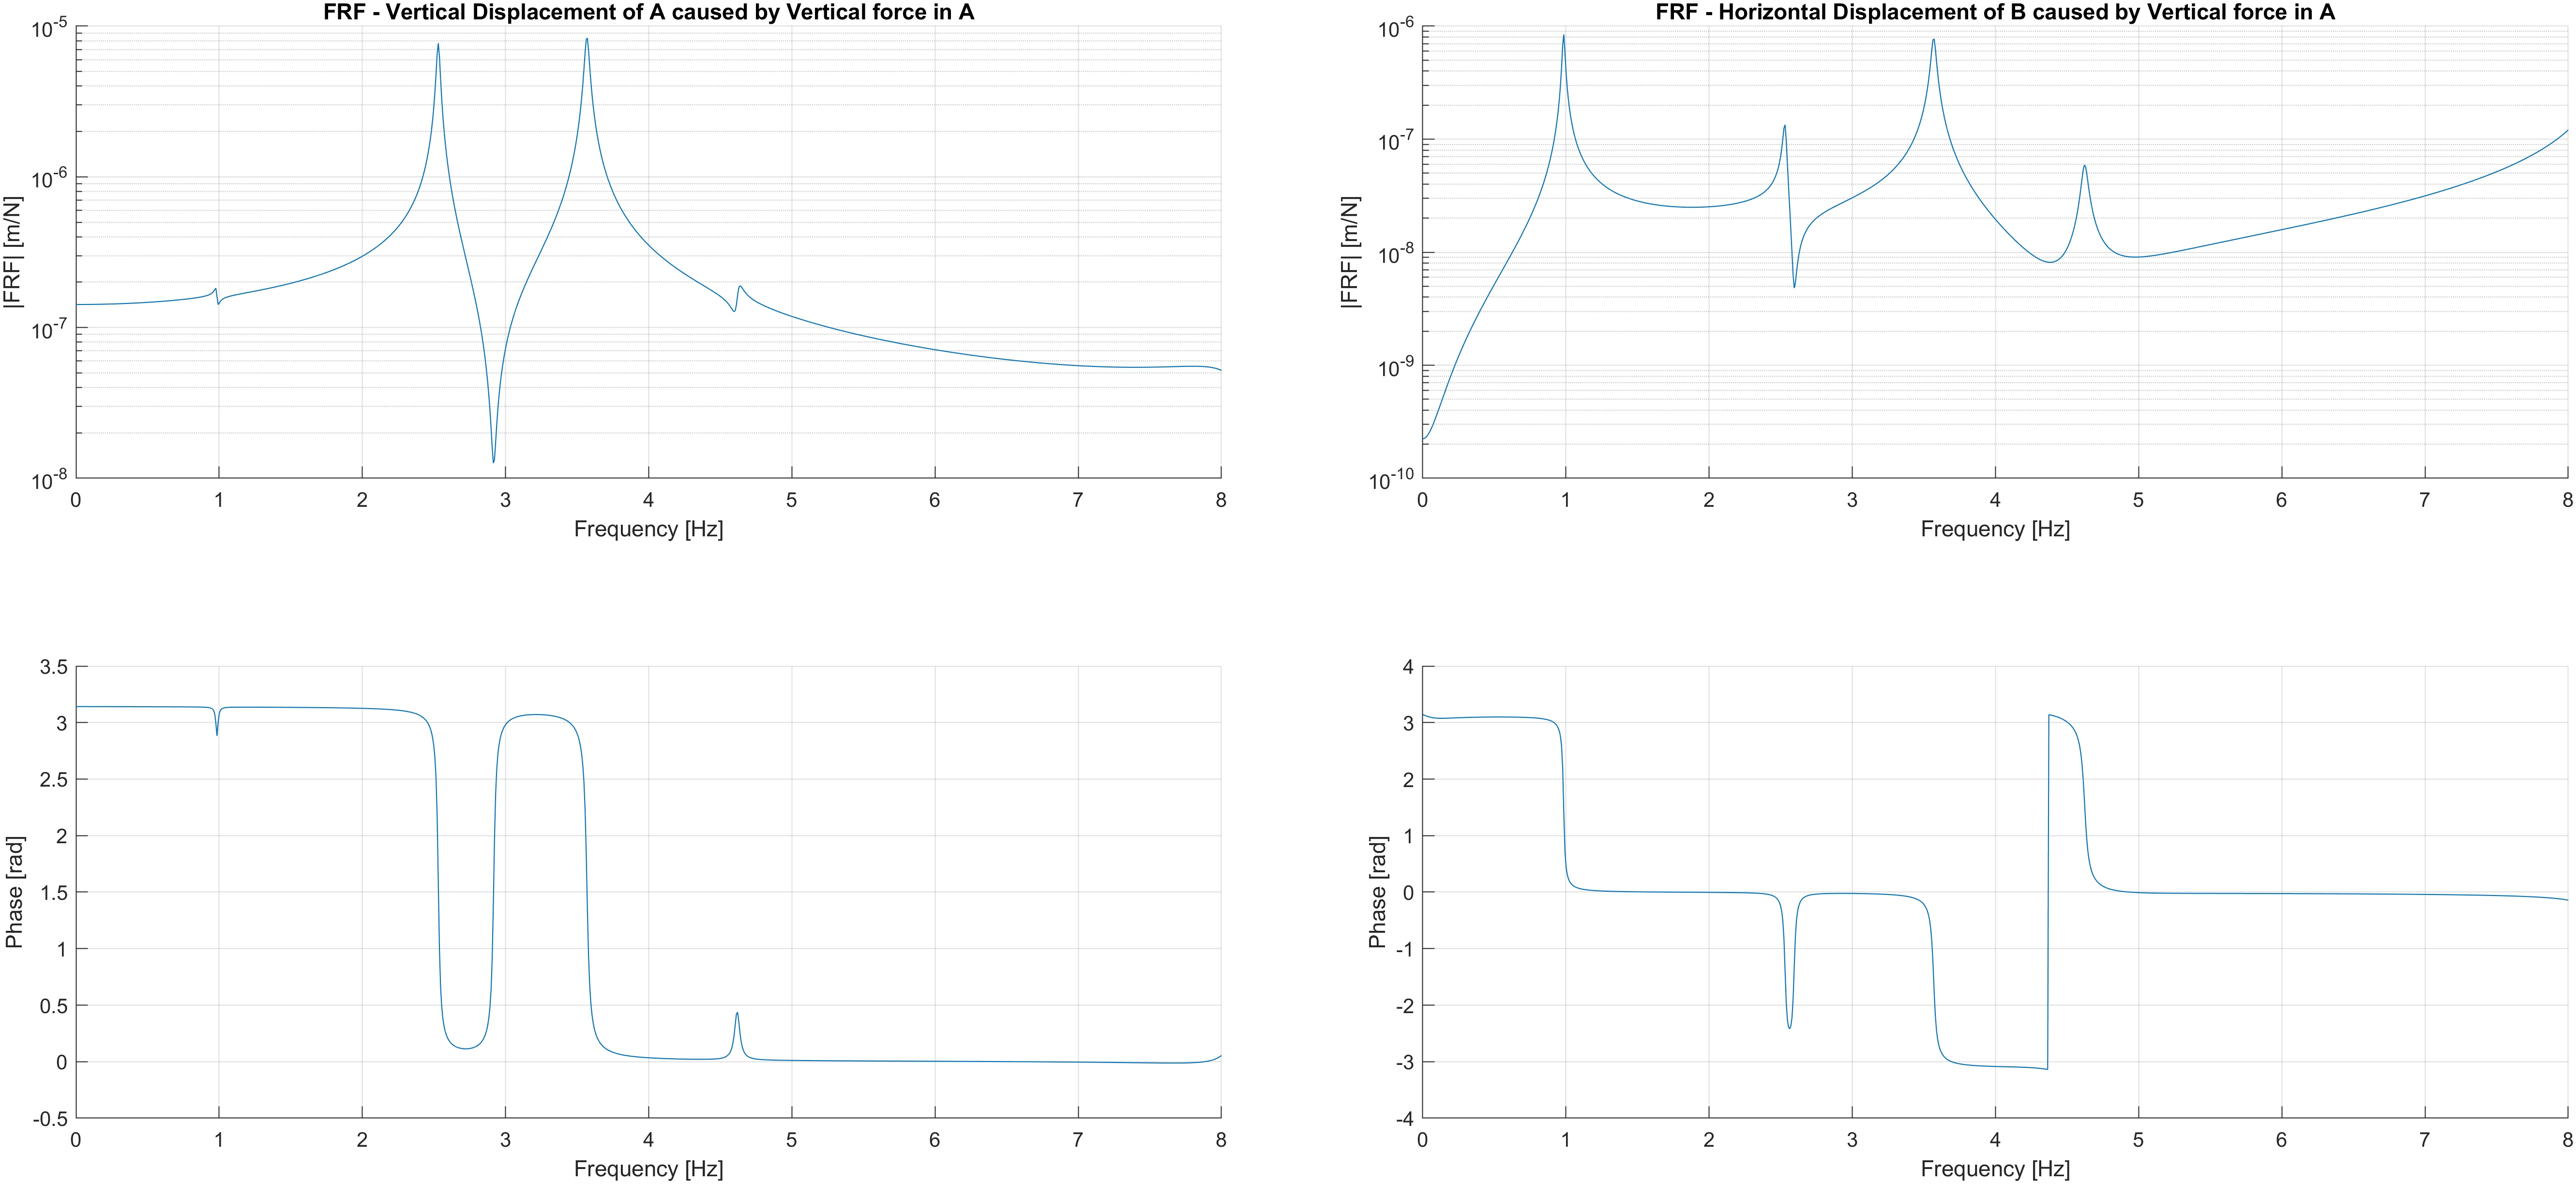
\includegraphics[width=\textwidth]{img/MATLAB/FRFs/Vertical_in_A.png}
    \caption{FRF computed using the direct method - Vertical force \textbf{A} to Vertical displacement \textbf{A} and Horizontal displacement \textbf{B}.}
    \label{fig:FRF_direct_vertical_A}
\end{figure}

From the FRFs shown in Figure \ref{fig:FRF_direct_vertical_A}, we can observe that in the considered frequency range ($0-8 [Hz]$), the vertical displacement of node \textbf{A} is more sensitive to the vertical force applied to node \textbf{A} than the horizontal displacement of node \textbf{B}.

Moreover, as expected, the resonance peaks in the FRFs correspond to the natural frequencies of the system found during modal analysis (see Section \ref{sub:modal_analysis}).

Interestingly, both FRFs exhibit an anti-resonance peak between the third and fourth natural frequencies (at $\approx 2.91 [Hz] \rightarrow 18.28 [rad/s]$), which indicates that the system's response to the excitation is minimized at that frequency.
In other words, at that specific excitation frequency, node \textbf{A} became stationary and any force applied at the corresponding frequency will not excite the system (no energy can flow from the force to the structure, null virtual work).


\subsubsection{Direct vs. Modal superposition method - Vertical force \textbf{A} to Horizontal displacement B}
\label{subsubsec:direct_vs_modal_vertical_force_A}

In this example, we compute the FRF relating the horizontal displacement of node \textbf{B} to the vertical force applied to node \textbf{A}.
We compare the results obtained using the direct method and the modal superposition method.

In order to have a significant comparison of the effect of the reduction of the number of modes considered in the analysis, we will consider only the first two mode shapes of the system in the modal superposition method ($n=2$).

\begin{figure}[H]
    \centering
    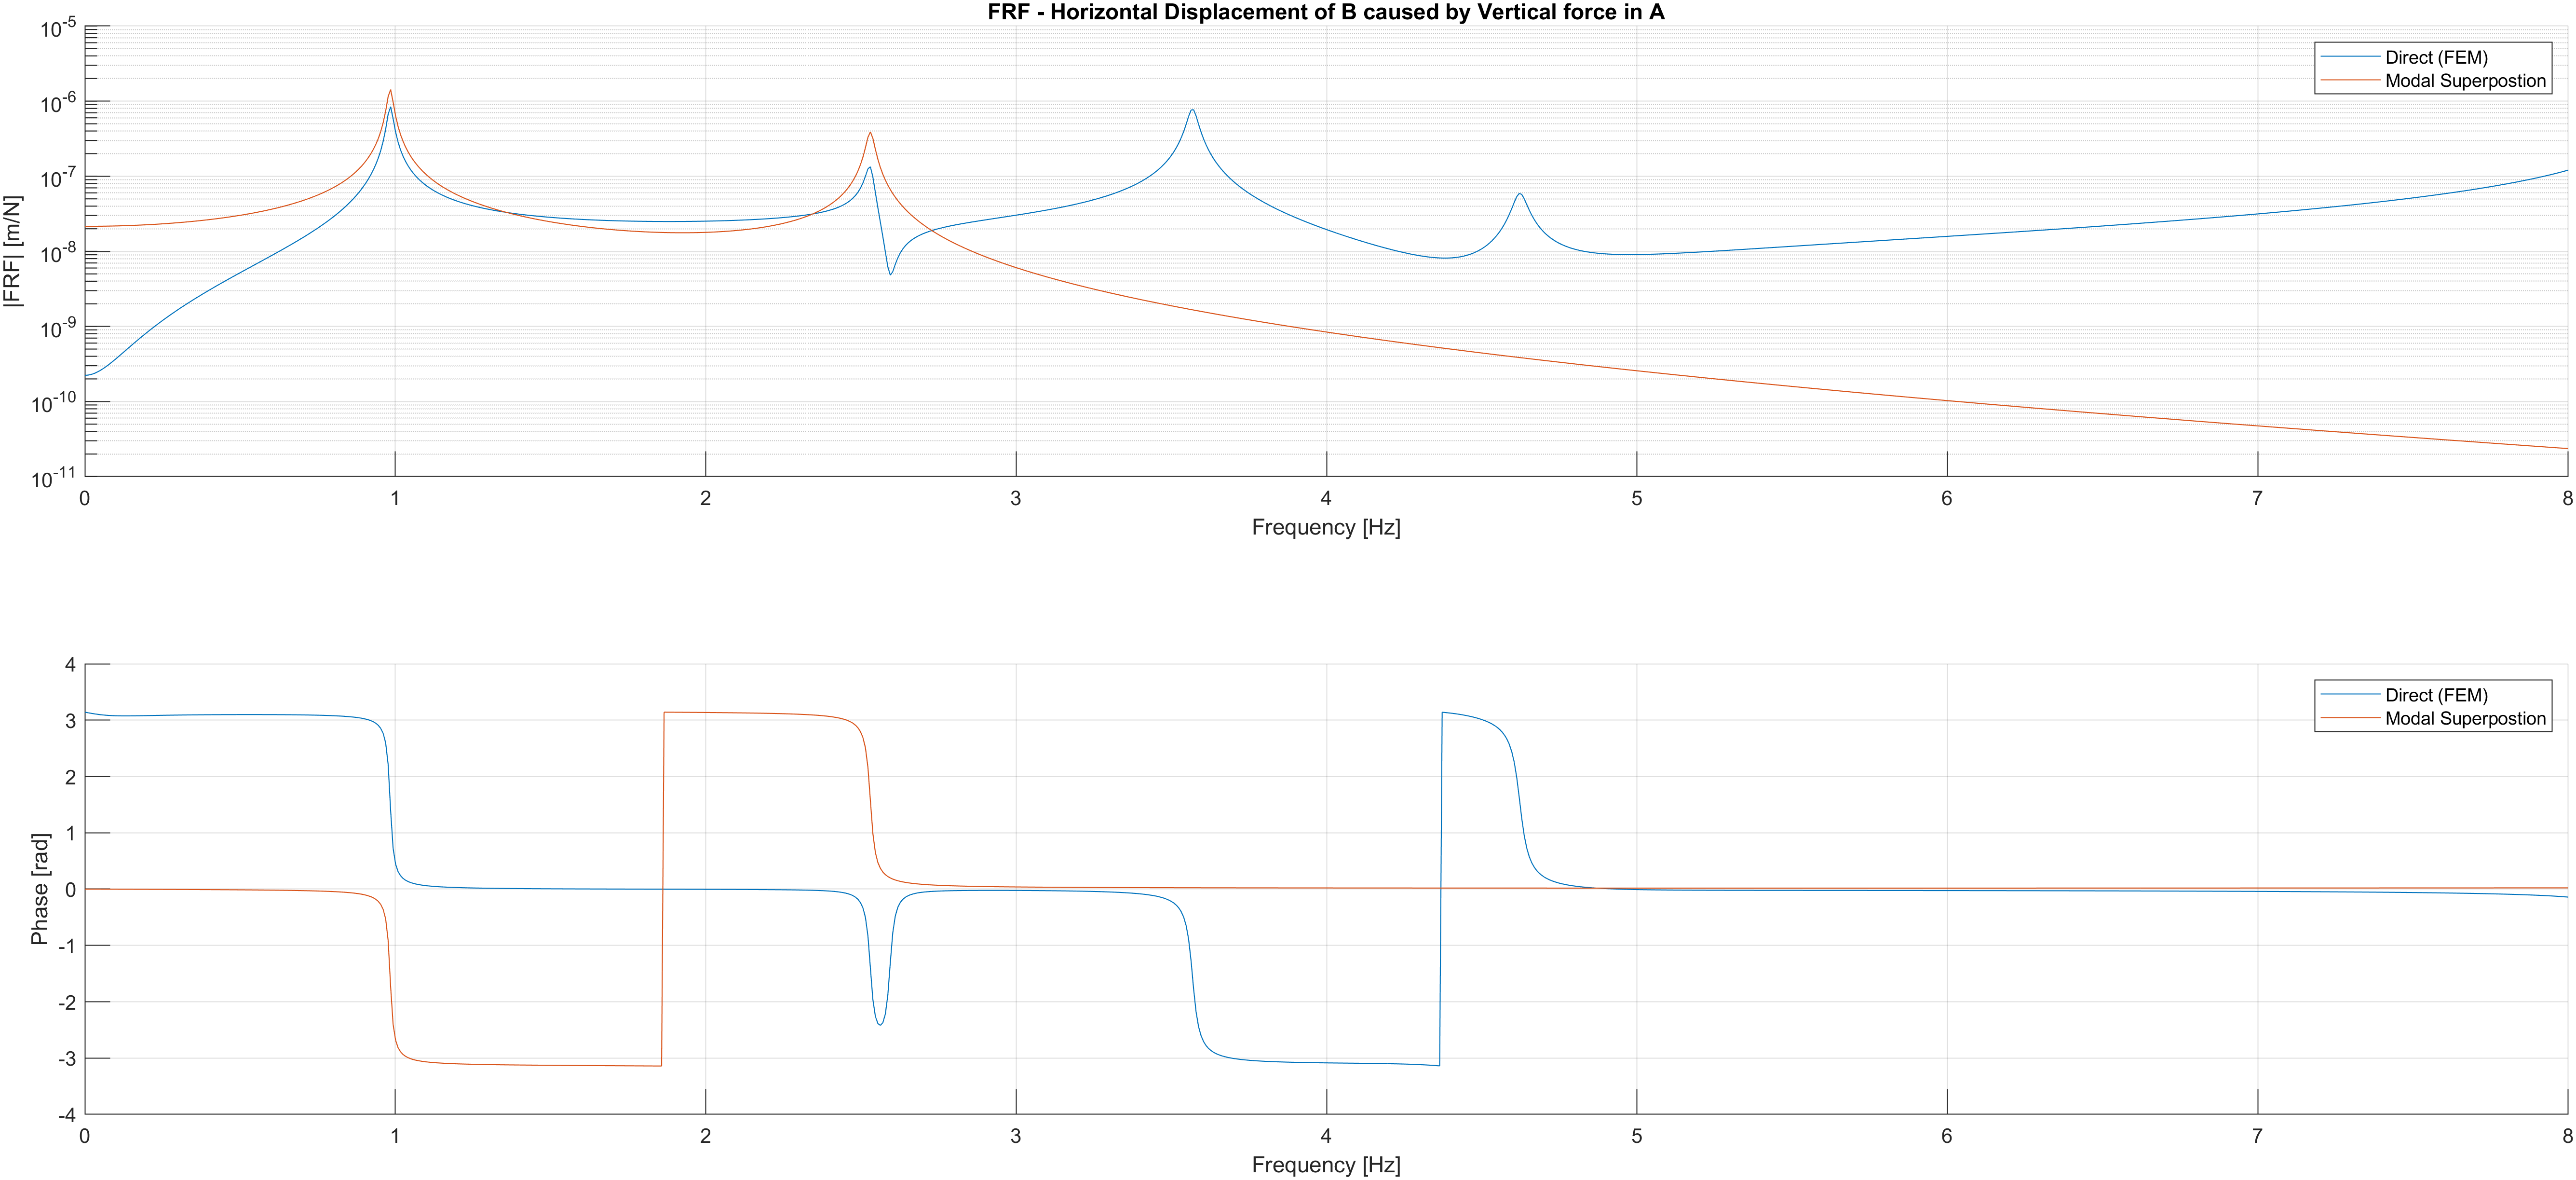
\includegraphics[width=\textwidth]{img/MATLAB/FRFs/Direct_vs_Modal.png}
    \caption{FRF computed using the direct method and modal superposition method - Vertical force \textbf{A} to Horizontal displacement \textbf{B}.}
    \label{fig:FRF_direct_vs_modal_vertical_A}
\end{figure}

From the FRFs shown in Figure \ref{fig:FRF_direct_vs_modal_vertical_A}, we can observe that the results obtained using the direct method and the modal superposition method are in good agreement only around the considered natural frequencies of the system.
As we move away from the peaks, the results start to diverge.

This behavior is expected since the modal superposition method considers only the first two mode shapes of the system, which may not capture the full dynamic behavior of the structure.
On the other hand, the direct method considers all the degrees of freedom of the system, providing a more accurate representation of the system's response to the excitation (at the cost of higher computational effort).


\subsubsection{Direct method - Vertical force \textbf{C} to Vertical reaction force \textbf{O2}}
\label{subsubsec:direct_method_vertical_force_C}

In this example, we compute the FRF relating the vertical reaction force at node \textbf{O2} to the vertical force applied to node \textbf{C}.
The FRF is computed using the direct method, considering all the degrees of freedom of the system.

\begin{figure}[H]
    \centering
    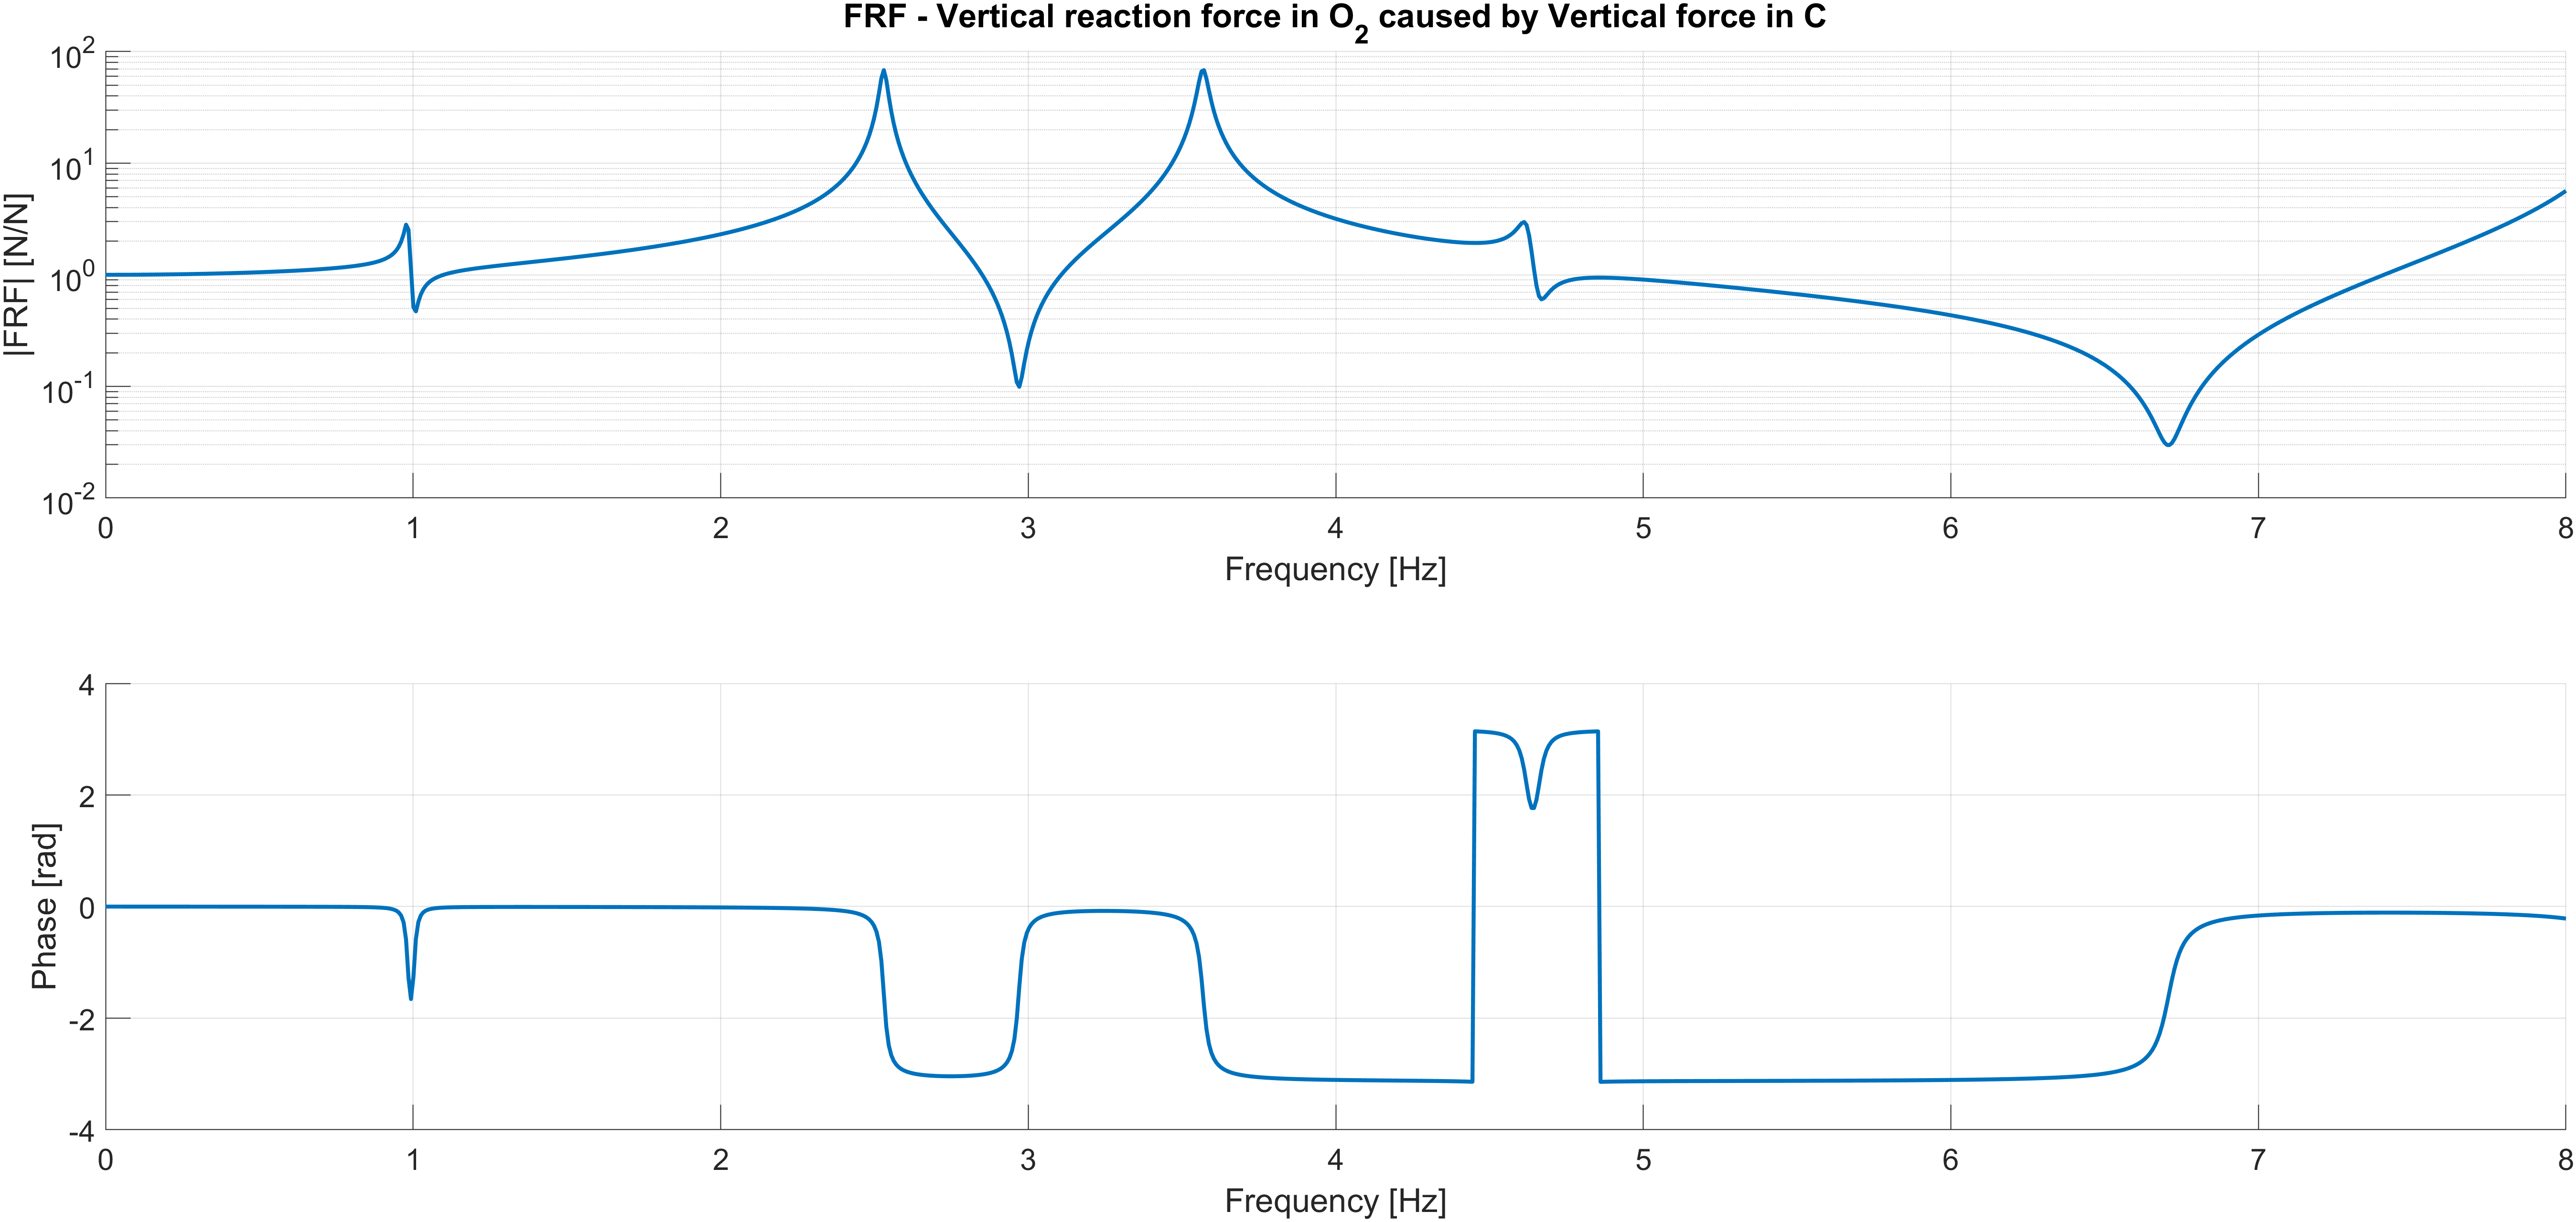
\includegraphics[width=\textwidth]{img/MATLAB/FRFs/Reaction_O2.png}
    \caption{FRF computed using the direct method - Vertical force \textbf{C} to Vertical reaction force \textbf{O2}}
    \label{fig:FRF_direct_vertical_C}
\end{figure}

Notice that reaction forces are computed in two consecutive steps: first, using the direct method the displacement in time of each node is computed obtaining the vector $\mathbf{q}(t)$, then the reaction forces are computed by substituting the displacement vector in the equation of motion relative to the constrained nodes, obtaining the reaction forces vector $\mathbf{R}(t)$.